\chapterimage{chapter_head_2.pdf} % Chapter heading image

\chapter{Caraterísticas da dança}

\begin{tcbinformation} 
\textbf{Dança:}
\index{Dança}
\label{def:DancaGeral}
Mas que uma simples palavra, a dança é um conceito; e como tal, esta representa 
uma ideia, juízo ou opinião; pelo que podemos ter múltiplas pontos de vista do que é a dança \cite[pp. 2]{Rejane2011}.
%Assim podemos listar os seguintes significados a palavra dança:
\begin{itemize}
\item ``Sequência de movimentos corporais executados de maneira ritmada, 
em geral ao som de música'' \cite[pp. 604]{ferreira1999novo}.
\item ``A arte de mover o corpo segundo a relação estabelecida entre tempo e espaço,
gerada pelo ritmo e a composição coreográfica'' \cite[pp. 17]{bencardinidanca}
\item A dança é a movimentação corporal, que tem como proposito, 
a expressão emocional, sentimental, lúdica ou artística.
%% correr para chegar ao otro lado exersicio, correr paa expresarse dança.
\end{itemize}
\end{tcbinformation} 

\begin{center}
\begin{tabular}{lll}
~ & Sim & Não \\
A dança é sempre feita com música? & \NoCheckedItem & \CheckedItem \\ %\hline
É necessário um par para dançar? & \NoCheckedItem & \CheckedItem \\ %\hline
A dança é uma arte? & \CheckedItem & \NoCheckedItem \\ %\hline
A dança tem necessariamente um significado? & \NoCheckedItem & \CheckedItem \\ %\hline 
%no confundir com: a dança tem um proposito? sim \cite[pp. 10]{schrader2005sense}
\end{tabular}
\end{center}

A primeira afirmação é fácil de entender, pois se neste momento ficamos em pé,
e iniciamos a contar, desde uma perspetiva emocional, a historia de nossa vida, 
utilizando nosso corpo e uma estrutura rítmica escolhida por nós mesmos,
então estaríamos sim dançando; porém sem música de fundo.

Do mesmo exemplo anterior se deduz que não necessitamos um par para nos expressar mediante a dança;
é mais, existem muitas disciplinas da dança em que não se necessita par,
por exemplo o ``free style''.

Seguindo o conceito presentado anteriormente, a dança sim é uma arte \cite[pp. 17]{bencardinidanca}.

A dança não tem que ter necessariamente um significado, 
pois podemos mover-nos ritmicamente pelo simples prazer de fazê-lo, 
sem nenhuma outra pretensão, 
ou também procurando ver o limite de nossas capacidades físicas.

%%%%%%%%%%%%%%%%%%%%%%%%%%%%%%%%%%%%%%%%%%%%%%%%%%%%%%%%%%%%%%%%%%%%%%%%%%%%%%%%
\input{chapters/cap-dance-elements/sec-dance-elements-elements}
%%%%%%%%%%%%%%%%%%%%%%%%%%%%%%%%%%%%%%%%%%%%%%%%%%%%%%%%%%%%%%%%%%%%%%%%%%%%%%%%

\section{Decorando passos de dança}
\label{sec:decorando-passos-de-danca}
Os professores de dança Aurélio e Neiliane,
mediante sua ``Escola de Dança on-line'' e seu projeto 
\href{https://www.facebook.com/dancandoeaprendendo/}{Dançando e Aprendendo}, 
entre outras muitas dicas de dança,
propõem
a utilização de uma \href{https://www.youtube.com/watch?v=ePwjQx5egAo}{``folha de memorização de passos''} 
para melhorar o aprendizado de passos de dança 
e a retenção destes na \hyperref[sec:memoria:longo]{\textbf{memória de longo prazo}}.

A proposta consiste em preencher uma destas folhas de memorização
por cada passo aprendido (ou em processo de aprender),
de modo que nela primeiro devemos colocar um título ou um nome de passo,
isto como um recurso mnemotécnico e para ajudar-nos a catalogar o passo em nosso acervo pessoal.
A folha também pede ao usuário uma descrição verbal do passo com luxo de detalhes, 
colocando estas informações como se fossem escritas para ser lidas por uma pessoa 
que não assistiu à aula onde ensinaram o passo; 
sendo esta uma forma em que você do presente pode enviar 
uma mensagem digerível e estruturada a você do futuro
sobre a mecânica de um passo de dança.
Outro item que pede a folha é agregar algum comentário que por associação 
te faça lembrar o movimento; por exemplo, no passo ``Romário'' se poderia anotar que 
o movimento é chamado assim porque se dá um chute, ou 
no movimento ``Puladinho'' pode-se anotar que este nome vem da frase ``para o ladinho'' pois no passo 
se vá para um lado e logo para outro.
Finalmente a folha recomenda ao usuário
ensinar o passo aprendido a um amigo imaginário,
com o fim de garantir que as informações antes escritas estejam completas 
e sejam coerentes.

\begin{tcbattention}
Na Pag. \pageref{pos:page:folhamemorizacao} 
podemos ver uma forma compacta da folha de memorização 
de passos proposta pelos professores Aurélio e Neiliane; porém,
recomendo fortemente ir ao 
\href{https://www.youtube.com/watch?v=ePwjQx5egAo}{sitio web}
dos professores para ver a forma extendida desta folha.
\end{tcbattention}

Além de todas estas indicações, 
propostas pelos professores Aurélio e Neiliane
na folha de memorização,
só agregaria que também deveriam ser anotadas referencias 
à data, o lugar e ao professor; pois um recurso como esta folha é muito importante
para contribuir com a documentação dos diferentes estilos, didáticas e informações
que podem ser achados na dança de salão no Brasil;
por exemplo, com o tempo uma pessoa poderia considerar que o conhecimento 
acumulado no seu acervo pode formar um livro, 
e este já estaria bem documentado e referenciado.

A folha de memorização de passos também atinge um ponto 
que foi a motivação principal para escrever este livro;
sendo esta, a necessidade de ter um método de notação coreográfica que permita, 
mediante símbolos e/ou texto, representar e descrever os movimentos executados
nos passos no samba de gafieira. Assim, 
a só existência da folha de memorização de passos, fomenta a ativação da 
inteligencia coletiva das pessoas que estão no mundo da dança 
a procurar ou criar algumas formas de notação coreográfica que permitam 
plasmar toda esta informação em palavra escrita.


 



\newpage
\thispagestyle{plain}
\begin{center}\TITULOA{Folha de memorização de passos}\end{center}
\label{pos:page:folhamemorizacao}

\begin{center}\Large\textit{ Esta folha é uma ferramenta simples de memorização e registro dos passos aprendidos.}\end{center}

\TITULOB{Nome do passo aprendido}
\noindent Digite no espaço o nome do passo que você aprendeu.

\BOXDATA\;

\TITULOB{Passo a passo} 
\noindent Descreva abaixo (com riqueza de detalhes) todo o passo a passo da
figura que você aprendeu. Descreva cada ação feita para realizar o passo.
É importante que sua anotação seja possível de ser entendida por outra 
pessoa além de você, portanto não economize nos detalhes do passo.

\LINEDATA\;
\LINEDATA\;
\LINEDATA\;
\LINEDATA\;
\LINEDATA

\TITULOB{Suas conexões}	
\noindent Escreva aqui que conexões (imagens cotidianas, histórias etc.)
você pode fazer para te ajudar a lembrar do passo que você acabou de aprender.
O que é presente no seu cotidiano que se você fizesse uma associação ao passo
te ajudaria a lembrar dele?

\LINEDATA\;
\LINEDATA\;
\LINEDATA

\TITULOB{Ensine ao amigo imaginário}
\noindent Para fechar o processo de aprendizado, ensine o passo que você aprendeu.
O ato de ensinar não só reforça o seu aprendizado como também te ajuda a
compreensão do passo, haja vista que para ensinar é necessário domínio do
que está sendo ensinado. Portanto, ensine o passo aprendido para o amigo 
imaginário.\\

\FOOTPAGE\;


%%%%%%%%%%%%%%%%%%%%%%%%%%%%%%%%%%%%%%%%%%%%%%%%%%%%%%%%%%%%%%%%%%%%%%%%%%%%%%%%
\section{Rota de estudo na danca de salão}
\label{sec:dance-elements-processo}
Nesta seção é presentada uma proposta de rota de estudo para o aprendizado da
dança de salão. 
Como mostra a Figura \ref{fig:dance-elements-processo},
a proposta está basejada em 3 níveis de trabalho.
\begin{figure}[!h]
\centering
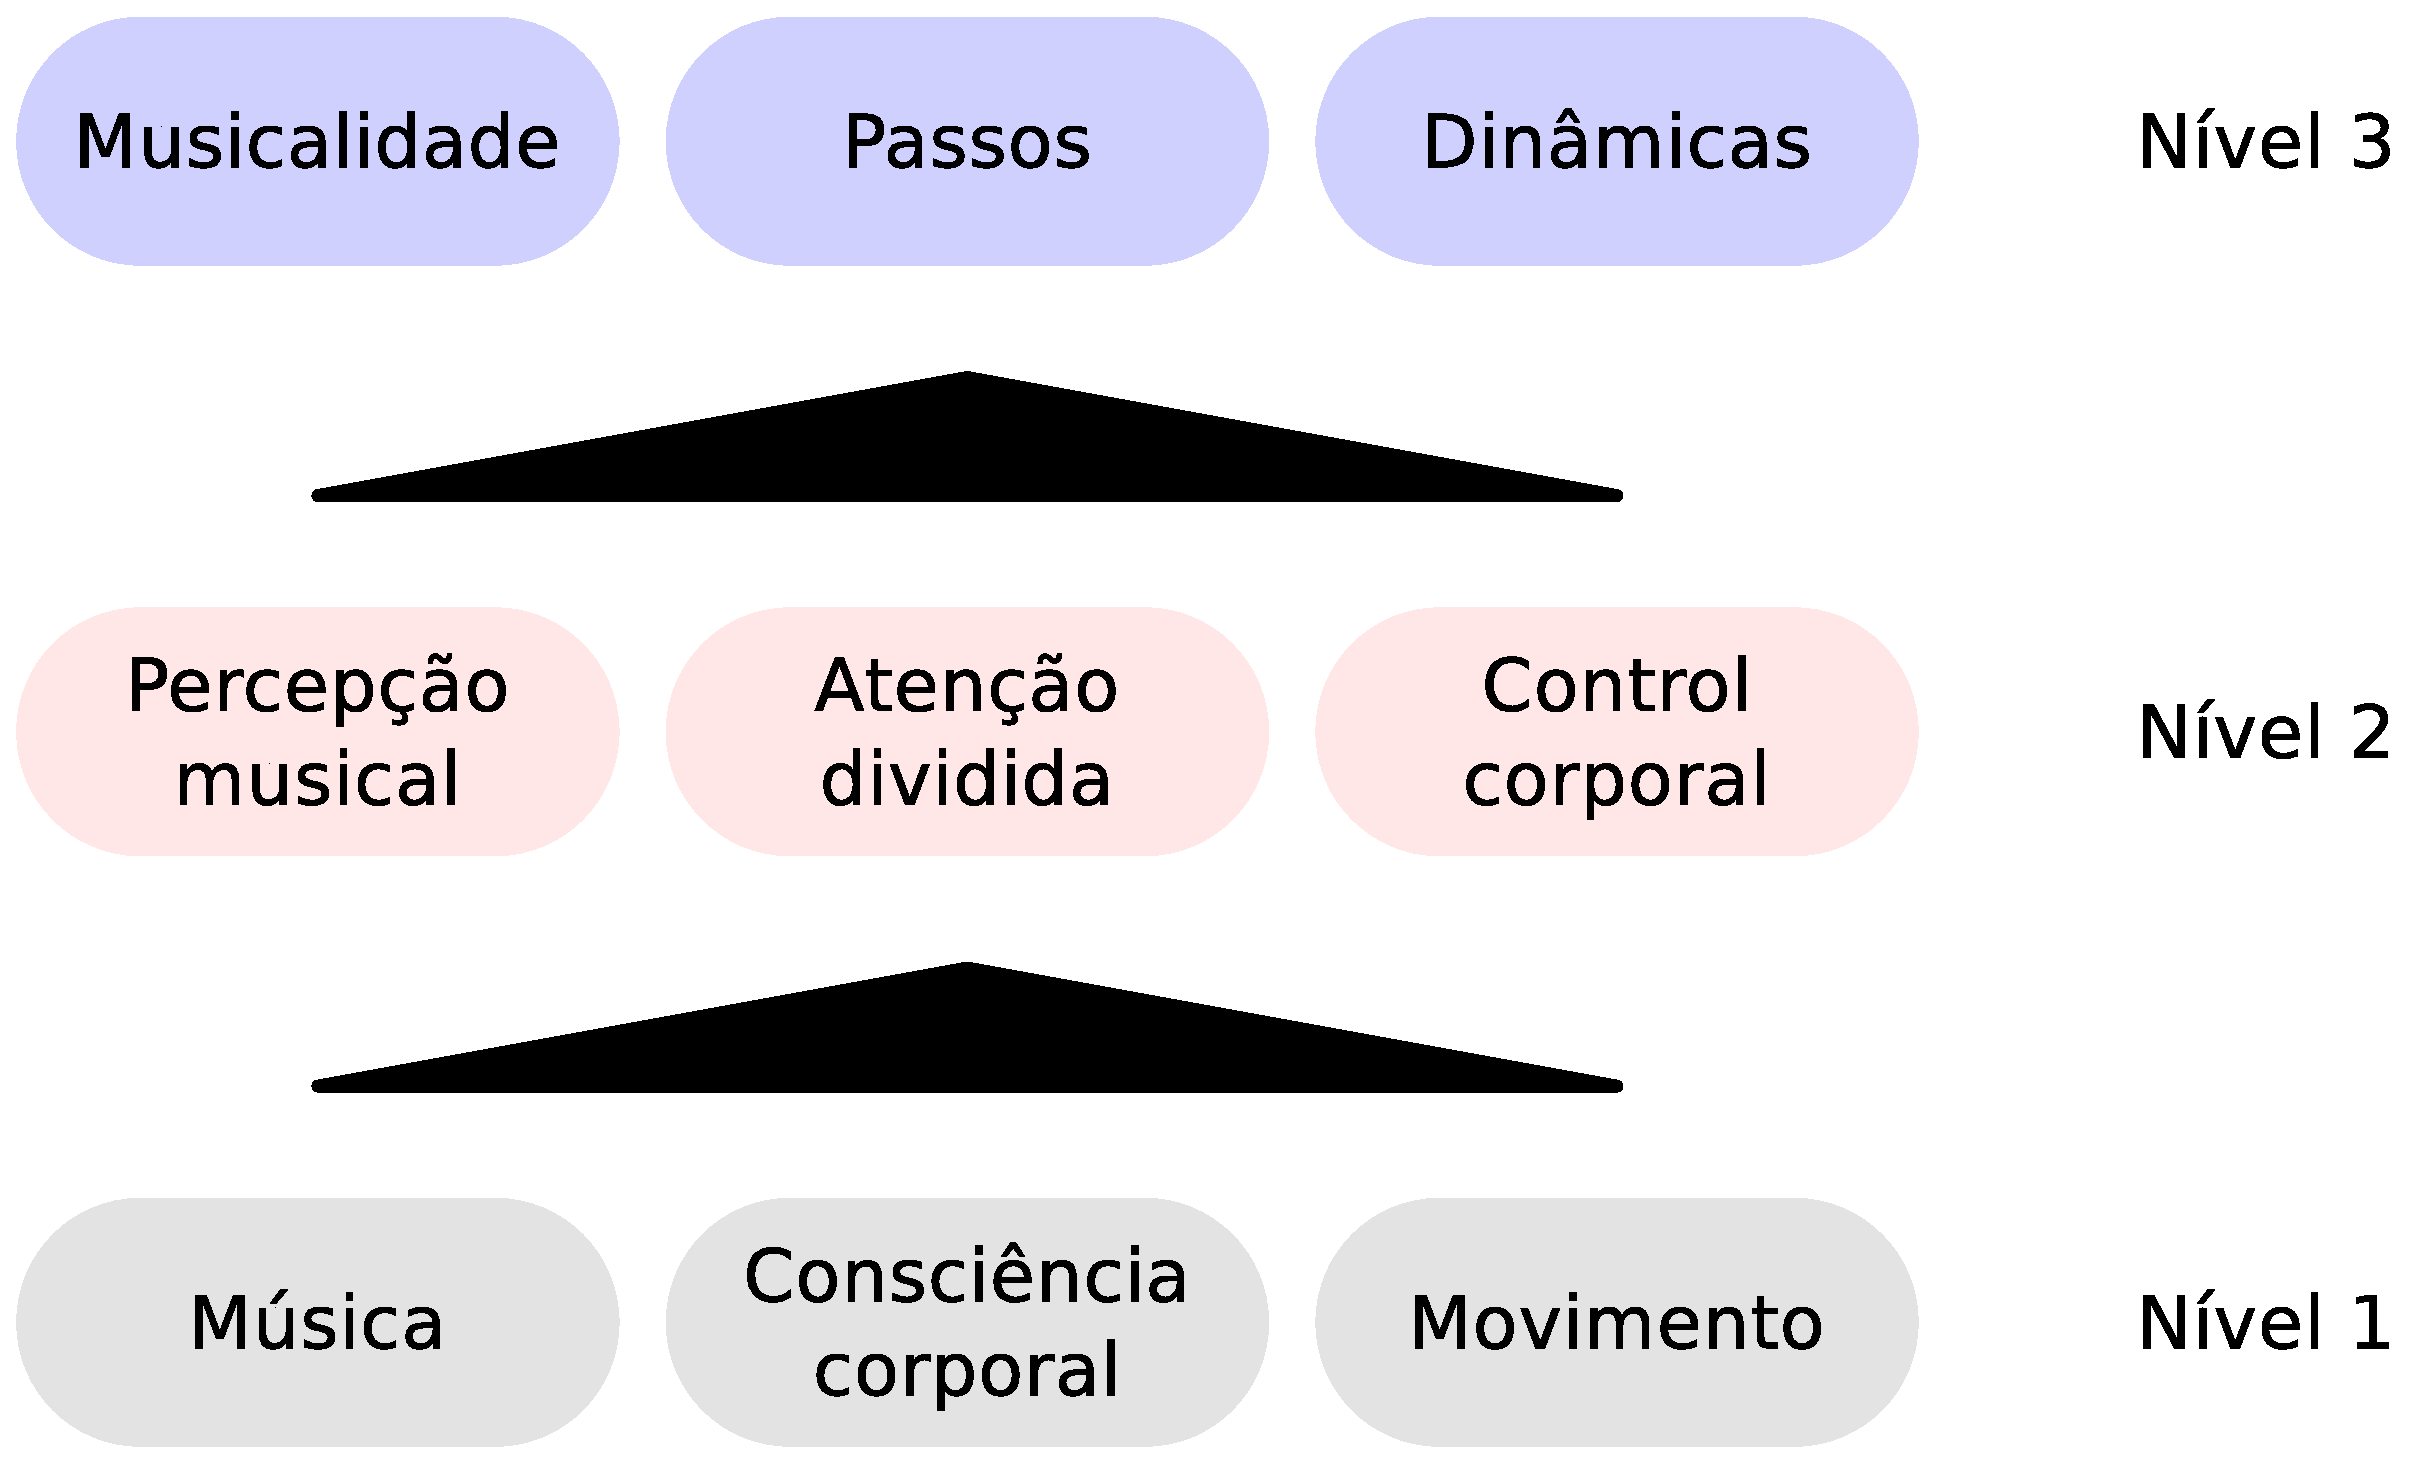
\includegraphics[width=0.7\textwidth]{chapters/cap-dance-elements/Diagrama-danca.eps}
\caption{Rota de estudo para o aprendizado da dança de salão.}
\label{fig:dance-elements-processo}
\end{figure}
\begin{itemize}
\item No nível 1 temos os temas mais básicos a serem estudados quando
iniciamos nosso percorrido na dança, estes são:
A teoria musical, a qual pode ser vista nos 
Capitulos \ref{cap:musicabasica}, \ref{cap:musicacomposer} e \ref{cap:musicatopicos}.
A consciência corporal, que é estudada no Capítulo \ref{fig:bodyrelations}.
O movimento, que corresponde ao aprimoramento de nossa aptidão física.
\item No nível 2 se inicia o perfeicionamento de habilidades,
mediante a combinação de vários componentes aprendidos no nível 1, estes são:
A percepção musical, a qual é vista no Capítulo \ref{cap:percepcaomusical}.
O controle corporal, que é estudado no Capítulo \ref{fig:bodyrelations}.
A atenção dividida, que é estudada nos Capítulos \ref{cap:aprendizagem} e \ref{chap:trainingbodycontrol}.
\item No nível 3 são listados os temas mais complexos os quais
requerem conhecimentos do nível 1 e/ou 2 para serem satisfatoriamente completados,
estes são:
A musicalidade, a qual é vista nos Capítulos \ref{chap:FundamentosMusicalidade} e \ref{chap:TopicosMusicalidade}.
As dinâmicas nos movimentos, que são estudadas na Seção \ref{sec:musicalidade:dinamicas}.
Os passos de dança, que são listados no Capítulo \ref{chap:passos-samba-gafieira}.
\end{itemize}
A proposta de estudo da Figura \ref{fig:dance-elements-processo} não aponta a que 
todo mundo deva inciar do nível 1, 
pois, dependendo da experiencia de vida de cada pessoa, estas podem ter conhecimentos de itens
em vários níveis no momento de iniciar seu aprendizado na dança de salão.
A proposta só busca dar uma orientação ao fluxo de estudos de um entusiasta à dança de salão.


